 \documentclass[a4paper,12pt]{article}
%%%%%%%%%%%%%%%%%%%%%%%%%%%%%%%%%%%%%%%%%%%%%%%%%%%%%%%%%%%%%%%%%%%%%%%%%%%%%%%%%%%%%%%%%%%%%%%%%%%%%%%%%%%%%%%%%%%%%%%%%%%%%%%%%%%%%%%%%%%%%%%%%%%%%%%%%%%%%%%%%%%%%%%%%%%%%%%%%%%%%%%%%%%%%%%%%%%%%%%%%%%%%%%%%%%%%%%%%%%%%%%%%%%%%%%%%%%%%%%%%%%%%%%%%%%%
\usepackage{eurosym}
\usepackage{vmargin}
\usepackage{amsmath}
\usepackage{multicol}
\usepackage{graphics}
\usepackage{epsfig}
\usepackage{subfigure}
\usepackage{fancyhdr}

\setcounter{MaxMatrixCols}{10}
%TCIDATA{OutputFilter=LATEX.DLL}
%TCIDATA{Version=5.00.0.2570}
%TCIDATA{<META NAME="SaveForMode" CONTENT="1">}
%TCIDATA{LastRevised=Wednesday, February 23, 2011 13:24:34}
%TCIDATA{<META NAME="GraphicsSave" CONTENT="32">}
%TCIDATA{Language=American English}

\pagestyle{fancy}
\setmarginsrb{20mm}{0mm}{20mm}{25mm}{12mm}{11mm}{0mm}{11mm}
\lhead{MA4413 2013} \rhead{Mr. Kevin O'Brien}
\chead{Addition to Formula Sheet }
%\input{tcilatex}

\begin{document}


\noindent \textbf{\textit{Binary Channels}}\\
Consider the binary channel in the figure below.
\begin{center}
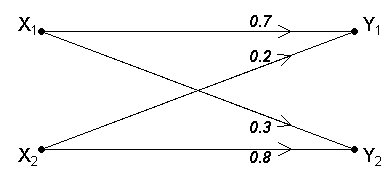
\includegraphics[scale=0.74]{10Bnet3}
\end{center}

\begin{itemize}
\item[(i)] Determine the channel matrix of the channel
\item[(ii)] Find $P(Y_1)$ and $P(Y_2)$ when $P(X_1) = 0.65$ and $P(X_2) = 0.35$.
\item[(iii)] Find the joint probabilities $P(X_1,Y_1)$ and $P(X_2,Y_2)$ when $P(X_1) = 0.65$ and $P(X_2) = 0.35$.
\end{itemize}
\end{itemize}


\end{document}